\documentclass{article}
\usepackage{ketpic,ketlayer}
\usepackage{amsmath,amssymb}
\usepackage{graphicx}
\usepackage{xcolor}
\usepackage{bm,enumerate}
\usepackage[colorlinks=true,urlcolor=blue]{hyperref}

\setmargin{20}{15}{15}{15}

\renewcommand{\labelitemi}{$\cdot$}

\pagestyle{empty}

\begin{document}

\begin{center}
Installing of KeTCindy 
\end{center}

\hfill Modified\ :\ \today

\begin{enumerate}[\bf\large 1.]
\item Install Cinderella, R, Maxima (and Sumatra only for Windows)
 \begin{itemize}
 \item \url{https://beta.cinderella.de}  (Cinderella)
 \item \url{https://cran.r-project.org}   (R)
 \item \url{https://sourceforge.net/projects/maxima/files}  (Maxima)
 \item \url{https://www.sumatrapdfreader.org/download-free-pdf-viewer.html} (Sumatra)\\
\hspace*{5mm}Rem) Sumatra should be installed in Program Files (or x86).
 \end{itemize}
\item Install a TeX system if no one has been installed.
 \begin{enumerate}[(1)]
 \item TeXLive is recommended.
    \begin{itemize}
    \item KeTCindy has been implemented (2018 or later).
    \end{itemize}
 \item KeTTeX is a light-weighted TeXLive.
    \begin{itemize}
    \item It is downloadable from\\
    \hspace*{5mm}Mac (kettex.dmg)\\
    \hspace*{10mm}\url{https://www.dropbox.com/s/dc4inuk06t07g26/kettex.dmg?dl=0}\\
    \hspace*{5mm}Windows (kettex.exe)\\
    \hspace*{10mm}\url{https://www.dropbox.com/s/fthw4btjqqs33tc/kettex.exe?dl=0}\\
    \hspace*{5mm}Linux (kettex.tar.xz)\\
    \hspace*{10mm}\url{https://www.dropbox.com/s/vg8p07832e9hzlk/KeTTeX-linux-20171022.tar.xz?dl=0}
     \item Move unzipped kettex into the folder /Applications for Mac and C:\textbackslash\ for Windows.
    \end{itemize}
 \end{enumerate}

\item Install KeTCindy
  \begin{enumerate}[(1)]
  \item Download ketcindy from CTAN(\url{https://ctan.org}).\\
  \hspace*{10mm}Search ketcindy $>$ Pack­age ketcindy $>$ Download\ \ ('ketcindy')
    \begin{itemize}
    \item[Rem)]The latest version is downloadable from Repository:\\
         \hspace*{5mm}Clone or download $>$ Download ZIP\ \ ('ketcindy-master')
    \end{itemize}
  \item Double click \verb|ketcindysettings.cdy| in the folder.
    \begin{itemize}
   \item  Select (1),(2) in the following figure, and execute (3) in order.
    \item Set Cinderella as the executive program if necessary.
    \item Reboot Cinderella if other cdy files are open.
   \end{itemize}
  \end{enumerate}

\vspace{2mm}

\begin{layer}{140}{0}
\putnotese{17}{20}{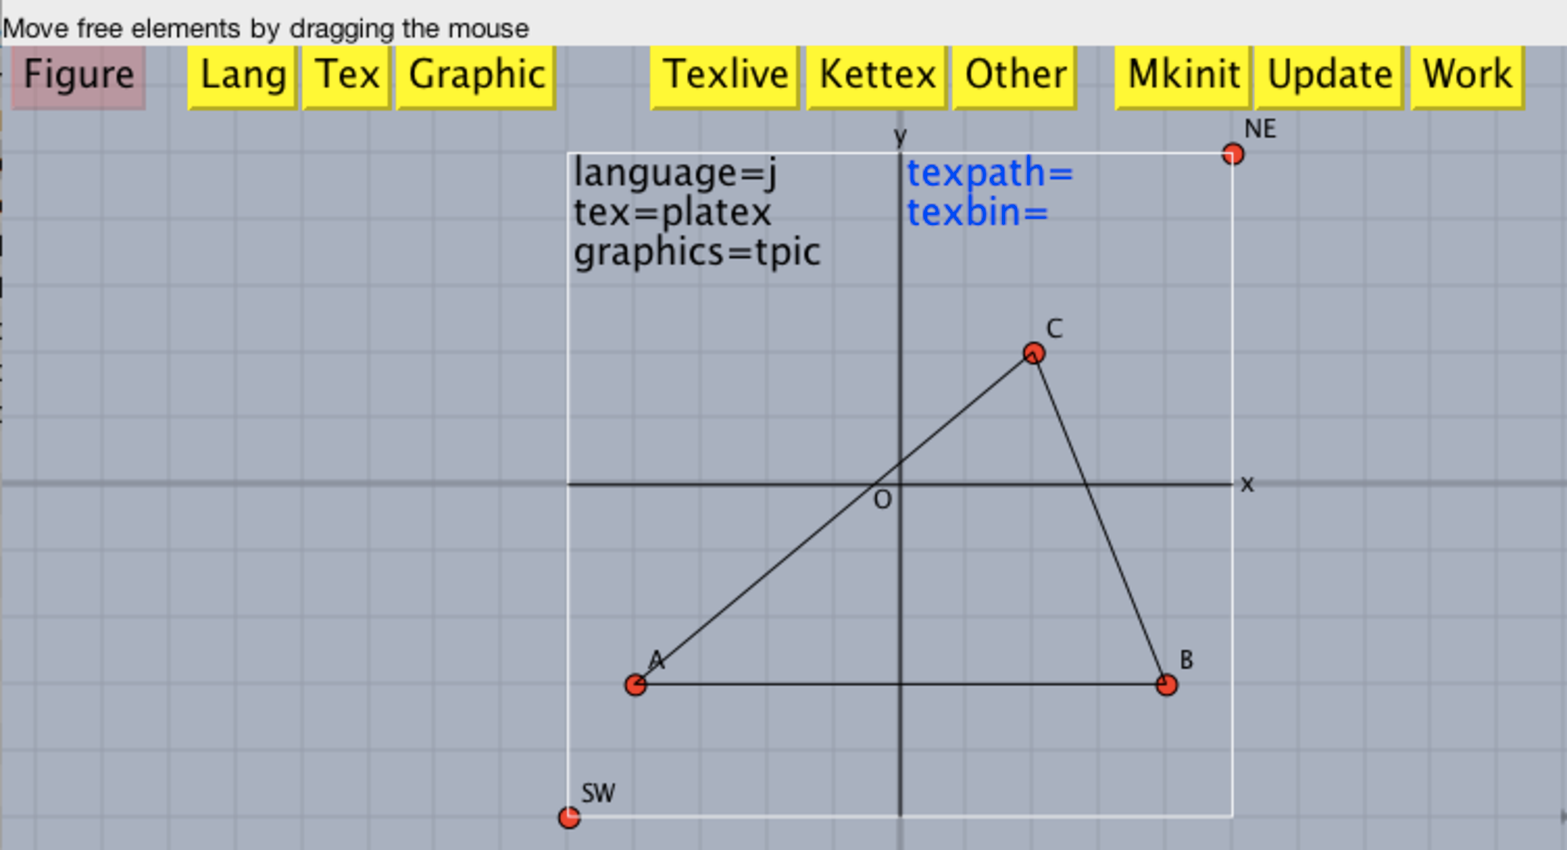
\includegraphics[bb=0.00 0.00 752.00 408.00,width=100mm]{Fig/setting.pdf}}
\putnotee{0}{5}{\bf [1]\ Select language,etc}
\putnotese{-7}{10}{\underline{Language}}
\putnotese{-3}{15}{Japanese, English}
\putnotese{-7}{20}{\underline{\TeX}}
\putnotese{-5}{24}{\begin{tabular}{l}
platex\\uplatex\\latex\\xelatex\\pdflatex\\lualatex\end{tabular}}
\putnotese{-7}{51}{\underline{Graphic Code}}
\putnotese{-5}{55}{\begin{tabular}{l}tpic\\pict2e\\tikz\end{tabular}}
\arrowline{37}{20}{17}{135}
\putnoten{73}{7}{\bf [2]Select \TeX\ sytem}
\arrowline{73}{20}{13}{90}
\putnotee{115}{5}{\bf [3]\ Folder operation}
\arrowline{100}{20}{20}{45}
\putnotese{121}{10}{\fbox{Mkinit}}
\putnotese{123}{17}{\begin{minipage}[t]{52mm}%
Create initialization file in user's home(Home).\hfill Name: ketcindy.ini
\end{minipage}}
\putnotese{121}{27}{\fbox{Update}}
\putnotese{123}{34}{Update ketcindy in \TeX\ system}
\putnotese{121}{40}{\fbox{Work}}
\putnotese{123}{47}{\begin{minipage}[t]{52mm}%
Create folder 'ketcindy' in Home.\\
Manuals, samples will be copied.
\end{minipage}}
\end{layer}

\vspace{75mm}

\item Test run
\begin{itemize}
\item Quit once Cinderella and double click \verb|ketcindytestrun.cdy|.
\item Press \verb|Figure| button, and the pdf will be displayed.
\item See Readmemore if errors occur.
\end{itemize}


  \end{enumerate}

\end{document}